\documentclass[12pt,a4paper]{article}
\usepackage[margin=1in]{geometry}
\usepackage{graphicx}
\usepackage{hyperref}
\usepackage{listings}
\usepackage{xcolor}
\usepackage{amsmath}
\usepackage{enumitem}
\usepackage{booktabs}
\usepackage{fancyhdr}
\usepackage{tikz}
\usetikzlibrary{shapes,arrows,positioning,fit,calc}

% Code listing style
\lstset{
    basicstyle=\ttfamily\small,
    breaklines=true,
    frame=single,
    backgroundcolor=\color{gray!10},
    keywordstyle=\color{blue}\bfseries,
    commentstyle=\color{green!60!black},
    stringstyle=\color{red!70!black},
    numbers=left,
    numberstyle=\tiny\color{gray},
    showstringspaces=false,
    tabsize=4,
    language=C++
}

\pagestyle{fancy}
\fancyhf{}
\rhead{2025201067}
\lhead{Secure P2P File Sharing}
\cfoot{\thepage}

\title{
    \vspace{-1cm}
    \textbf{Secure Peer-to-Peer File Sharing System} \\
    \large Advanced Operating Systems --- Assignment 3 \\
    \large Systems \& Network Security Integration
}
\author{
    \textbf{Roll Number:} 2025201067 \\
    IIIT Hyderabad
}
\date{Monsoon 2025}

\begin{document}
\maketitle
\tableofcontents
\newpage

% ============================================================
\section{Abstract}
% ============================================================

This report presents the design and implementation of a \textbf{secure peer-to-peer (P2P) file sharing system} inspired by BitTorrent. Unlike traditional P2P systems that transmit data in plaintext, our system integrates a comprehensive security layer consisting of:

\begin{itemize}
    \item \textbf{TLS 1.2+} encryption on all communication channels
    \item \textbf{Mutual TLS (mTLS)} with X.509 certificates for peer authentication
    \item \textbf{RSA-2048 digital signatures} on file metadata to prevent tampering
    \item \textbf{SHA-256} cryptographic hashing for file integrity verification
    \item \textbf{Salted password hashing} to protect stored credentials
    \item A full \textbf{PKI (Public Key Infrastructure)} with the tracker acting as a Certificate Authority
\end{itemize}

The system supports multi-seeder downloads with a rarest-piece-first strategy, partial file serving, and two-tracker redundancy with automatic state synchronization.

% ============================================================
\section{System Architecture}
% ============================================================

\subsection{High-Level Overview}

The system consists of three types of entities:

\begin{enumerate}
    \item \textbf{Tracker (Server):} Centralized coordination server managing user accounts, groups, file metadata, seeder information, and acting as a Certificate Authority (CA).
    \item \textbf{Client:} Peer application that uploads, downloads, and shares files. Each client runs an embedded peer server.
    \item \textbf{Certificate Authority:} Embedded within the tracker; issues X.509 certificates to authenticated users.
\end{enumerate}

\subsection{Architecture Diagram}

\begin{center}
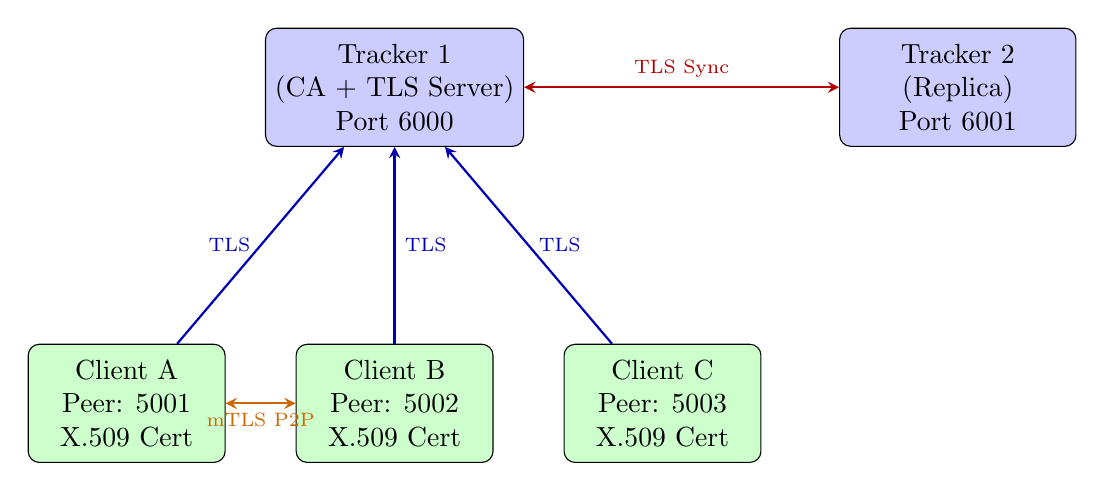
\begin{tikzpicture}[
    node distance=1.5cm,
    server/.style={rectangle, draw, fill=blue!20, minimum width=3cm, minimum height=1.5cm, align=center, rounded corners},
    client/.style={rectangle, draw, fill=green!20, minimum width=2.5cm, minimum height=1.5cm, align=center, rounded corners},
    arrow/.style={->, thick, >=stealth},
    darrow/.style={<->, thick, >=stealth}
]
    \node[server] (t1) {Tracker 1\\(CA + TLS Server)\\Port 6000};
    \node[server, right=4cm of t1] (t2) {Tracker 2\\(Replica)\\Port 6001};
    
    \node[client, below left=2.5cm and 0.5cm of t1] (c1) {Client A\\Peer: 5001\\X.509 Cert};
    \node[client, below=2.5cm of t1] (c2) {Client B\\Peer: 5002\\X.509 Cert};
    \node[client, below right=2.5cm and 0.5cm of t1] (c3) {Client C\\Peer: 5003\\X.509 Cert};
    
    \draw[darrow, red!70!black] (t1) -- node[above] {\scriptsize TLS Sync} (t2);
    \draw[arrow, blue!70!black] (c1) -- node[left, font=\scriptsize] {TLS} (t1);
    \draw[arrow, blue!70!black] (c2) -- node[right, font=\scriptsize] {TLS} (t1);
    \draw[arrow, blue!70!black] (c3) -- node[right, font=\scriptsize] {TLS} (t1);
    \draw[darrow, orange!80!black] (c1) -- node[below, font=\scriptsize] {mTLS P2P} (c2);
\end{tikzpicture}
\end{center}

\subsection{Communication Channels}

\begin{table}[h]
\centering
\begin{tabular}{@{}lll@{}}
\toprule
\textbf{Channel} & \textbf{Security} & \textbf{Purpose} \\
\midrule
Client $\leftrightarrow$ Tracker & TLS 1.2+ (server auth) & Commands, metadata, cert issuance \\
Client $\leftrightarrow$ Client & mTLS (mutual auth) & Piece transfer, bitmap queries \\
Tracker $\leftrightarrow$ Tracker & TLS 1.2+ & State synchronization \\
\bottomrule
\end{tabular}
\caption{Communication channels and their security properties}
\end{table}

% ============================================================
\section{Security Design}
% ============================================================

\subsection{Threat Model}

We consider the following threats:

\begin{enumerate}
    \item \textbf{Eavesdropping:} An attacker on the network can observe all traffic between any two entities.
    \item \textbf{Man-in-the-Middle (MitM):} An attacker can intercept and modify messages in transit.
    \item \textbf{Impersonation:} A malicious node can pretend to be a legitimate peer to serve corrupted file pieces.
    \item \textbf{Metadata Tampering:} A compromised tracker could alter piece hashes to redirect downloads to malware.
    \item \textbf{Credential Theft:} An attacker with access to the tracker's memory could steal user passwords.
\end{enumerate}

\subsection{Mitigation Summary}

\begin{table}[h]
\centering
\begin{tabular}{@{}lll@{}}
\toprule
\textbf{Threat} & \textbf{Mitigation} & \textbf{Mechanism} \\
\midrule
Eavesdropping & Channel encryption & TLS 1.2+ (AES-256-GCM) \\
MitM & Server authentication & X.509 certificates, CA verification \\
Impersonation & Peer authentication & Mutual TLS with tracker-issued certs \\
Metadata Tampering & Digital signatures & RSA-2048 with SHA-256 digest \\
Credential Theft & Password hashing & SHA-256(salt $\|$ password) \\
\bottomrule
\end{tabular}
\caption{Threat mitigations implemented in the system}
\end{table}

\subsection{TLS 1.2+ Encryption}

All TCP connections in the system are wrapped with TLS using OpenSSL. The implementation uses:

\begin{itemize}
    \item \texttt{TLS\_server\_method()} and \texttt{TLS\_client\_method()} for version-agnostic TLS
    \item Minimum protocol version set to TLS 1.2 via \texttt{SSL\_CTX\_set\_min\_proto\_version()}
    \item Server certificate verification via \texttt{SSL\_CTX\_load\_verify\_locations()} with the CA cert
\end{itemize}

\begin{lstlisting}[caption={TLS Context Creation (Server Side)},label=lst:tls-server]
SSL_CTX* create_server_tls_ctx(const char* cert, 
                                const char* key, 
                                const char* ca) {
    SSL_CTX* ctx = SSL_CTX_new(TLS_server_method());
    SSL_CTX_set_min_proto_version(ctx, TLS1_2_VERSION);
    SSL_CTX_use_certificate_file(ctx, cert, SSL_FILETYPE_PEM);
    SSL_CTX_use_PrivateKey_file(ctx, key, SSL_FILETYPE_PEM);
    SSL_CTX_load_verify_locations(ctx, ca, nullptr);
    SSL_CTX_set_verify(ctx, SSL_VERIFY_PEER, nullptr);
    return ctx;
}
\end{lstlisting}

\subsection{PKI and Certificate Management}

The system implements a complete PKI chain:

\begin{enumerate}
    \item \textbf{Certificate Authority (CA):} A self-signed RSA-2048 root certificate generated by \texttt{generate\_certs.sh}. The CA's private key is loaded by the tracker at startup.
    
    \item \textbf{Tracker Certificate:} An X.509 certificate signed by the CA, presented to clients during TLS handshake. Clients verify this certificate against the CA cert.
    
    \item \textbf{Client Certificates (On-the-fly):} When a user successfully logs in, the tracker:
    \begin{enumerate}
        \item Generates a new RSA-2048 key pair for the client
        \item Creates an X.509 certificate with \texttt{CN=<username>}
        \item Signs it with the CA's private key using SHA-256
        \item Sends the PEM-encoded certificate and private key to the client over the TLS channel
    \end{enumerate}
\end{enumerate}

\begin{lstlisting}[caption={On-the-fly Certificate Generation (Tracker)},label=lst:cert-gen]
// Generate RSA-2048 key pair for client
EVP_PKEY* client_key = EVP_PKEY_new();
RSA* rsa = RSA_generate_key(2048, RSA_F4, NULL, NULL);
EVP_PKEY_assign_RSA(client_key, rsa);

// Create X509 certificate
X509* cert = X509_new();
X509_set_version(cert, 2); // v3
X509_NAME* name = X509_get_subject_name(cert);
X509_NAME_add_entry_by_txt(name, "CN", MBSTRING_ASC, 
    (unsigned char*)username.c_str(), -1, -1, 0);

// Sign with CA key (SHA-256 digest)
X509_sign(cert, ca_key, EVP_sha256());
\end{lstlisting}

\subsection{Mutual TLS (mTLS) for P2P}

When Client A wants to download a piece from Client B:

\begin{enumerate}
    \item Client A connects to Client B's peer server via TCP
    \item Both sides perform a TLS handshake presenting their X.509 certificates
    \item Each side verifies the peer's certificate is signed by the trusted CA
    \item If verification fails, the connection is rejected
    \item Piece data is transferred over the encrypted, authenticated channel
\end{enumerate}

This prevents unauthorized peers from joining the swarm and serving malicious pieces.

\subsection{RSA-2048 Digital Signatures}

File metadata integrity is protected by RSA-2048 digital signatures:

\begin{enumerate}
    \item \textbf{Upload:} The client constructs a metadata blob: \\
    \texttt{filename|filesize|file\_hash|piece\_hash\_1|...|piece\_hash\_N}
    
    \item \textbf{Signing:} The client computes \texttt{RSA\_Sign(SHA256(metadata\_blob), private\_key)}
    
    \item \textbf{Storage:} The hex-encoded signature and the client's public key are sent to the tracker along with the file metadata.
    
    \item \textbf{Verification:} When another client requests a download, the tracker includes the signature and public key in the response. The downloader verifies: \\
    \texttt{RSA\_Verify(SHA256(metadata\_blob), signature, public\_key)}
\end{enumerate}

\begin{lstlisting}[caption={RSA-2048 Digital Signature},label=lst:rsa-sign]
string rsa_sign(const string& priv_pem, const string& data) {
    // Load private key from PEM
    BIO* bio = BIO_new_mem_buf(priv_pem.c_str(), -1);
    EVP_PKEY* pkey = PEM_read_bio_PrivateKey(bio, ...);
    
    // Sign with SHA-256 digest
    EVP_MD_CTX* ctx = EVP_MD_CTX_new();
    EVP_SignInit(ctx, EVP_sha256());
    EVP_SignUpdate(ctx, data.c_str(), data.size());
    EVP_SignFinal(ctx, sig_buf, &sig_len, pkey);
    
    return hex_encode(sig_buf, sig_len);
}
\end{lstlisting}

\subsection{Salted Password Hashing}

Passwords are never stored in plaintext on the tracker:

\begin{enumerate}
    \item \textbf{Registration:} A random 16-byte salt is generated using \texttt{RAND\_bytes()}. The password is hashed as \texttt{SHA256(salt $\|$ password)} and stored alongside the salt.
    
    \item \textbf{Login:} The provided password is hashed with the stored salt and compared against the stored hash.
    
    \item \textbf{Sync:} The hashed password and salt (not the plaintext) are synchronized to the peer tracker.
\end{enumerate}

This means even if an attacker gains access to the tracker's memory, they cannot recover plaintext passwords.

\subsection{SHA-256 File Integrity}

All file integrity verification uses SHA-256 (replacing the cryptographically broken SHA-1):

\begin{itemize}
    \item \textbf{Piece-level:} Each 512KB chunk is independently hashed with SHA-256 during upload. During download, each received piece is re-hashed and compared against the expected hash.
    \item \textbf{Full-file:} A streaming SHA-256 hash of the entire file is computed during upload using \texttt{SHA256\_Init/Update/Final}, processing chunks sequentially without loading the full file into memory.
    \item \textbf{Hash length:} 64 hexadecimal characters (256 bits) vs.\ SHA-1's 40 characters (160 bits).
\end{itemize}

% ============================================================
\section{Network Protocol Design}
% ============================================================

\subsection{Client $\leftrightarrow$ Tracker Protocol (over TLS)}

All messages are newline-terminated and transmitted over TLS-encrypted channels.

\begin{table}[h]
\centering
\small
\begin{tabular}{@{}p{5cm}p{7cm}@{}}
\toprule
\textbf{Request} & \textbf{Response} \\
\midrule
\texttt{create\_user <uid> <pwd>} & \texttt{User created successfully} \\
\texttt{login <uid> <pwd> <ip:port>} & \texttt{Login successful CERT <hex> KEY <hex>} \\
\texttt{UPLOAD\_FILE <gid> <fname> <size> <hash> <pieces> <sig> <pubkey>} & \texttt{SUCCESS: File metadata uploaded} \\
\texttt{DOWNLOAD\_FILE <gid> <fname>} & \texttt{DOWNLOAD\_INFO <size> <seeders> <hashes> SIG <sig> PUBKEY <pubkey>} \\
\bottomrule
\end{tabular}
\caption{Key protocol messages (security-relevant fields highlighted)}
\end{table}

\subsection{Peer-to-Peer Protocol (over mTLS)}

Each piece request uses a short-lived mTLS connection:

\begin{itemize}
    \item \texttt{GET\_PIECE <filename> <index>} $\rightarrow$ \texttt{PIECE\_LEN <bytes>} + raw data
    \item \texttt{GET\_BITMAP <filename> <total>} $\rightarrow$ \texttt{BITMAP <bitstring>}
\end{itemize}

% ============================================================
\section{Key Algorithms}
% ============================================================

\subsection{Rarest Piece First}

Before downloading, the client queries all seeders for their piece bitmaps:

\begin{enumerate}
    \item For each seeder, send \texttt{GET\_BITMAP} and receive a binary string (e.g., \texttt{"110101"})
    \item Compute rarity: for each piece, count how many seeders have it
    \item Worker threads select the piece with the \textbf{lowest rarity} (fewest sources)
    \item A random seeder is chosen from those that have the selected piece
\end{enumerate}

This strategy ensures rare pieces are replicated first, preventing the ``last piece'' problem.

\subsection{Multi-Threaded Download Engine}

\begin{itemize}
    \item Thread count = $\min(\text{hardware\_concurrency}, \text{total\_pieces})$
    \item Each worker independently claims a piece (under mutex), downloads it via mTLS, verifies its SHA-256 hash, and writes to disk using \texttt{pwrite()} at the correct byte offset
    \item Failed pieces are retried up to 5 times before aborting
    \item A \texttt{condition\_variable} coordinates completion between workers and the manager thread
\end{itemize}

% ============================================================
\section{Data Structures}
% ============================================================

\subsection{Tracker Side}

\begin{lstlisting}[caption={Core Data Structures (Tracker)}]
struct User {
    string username;
    string password;      // SHA-256 hash (never plaintext)
    string password_salt; // 16-byte random salt (hex)
    bool logged_in;
    string ip; int port;
};

struct FileMetadata {
    size_t filesize;
    string file_hash;           // SHA-256 of full file
    vector<string> piece_hashes; // SHA-256 per 512KB chunk
    vector<string> seeders;
    string signature;           // RSA-2048 digital signature
    string uploader_pubkey;     // Uploader's RSA public key
};

struct Group {
    string group_id, owner;
    vector<string> members, pending_requests;
    map<string, FileMetadata> files;
};
\end{lstlisting}

\subsection{Client Side}

\begin{lstlisting}[caption={Download State (Client)}]
struct DownloadState {
    vector<PieceStatus> piece_status; // NEEDED/IN_FLIGHT/HAVE
    atomic<int> pieces_completed;
    vector<string> seeder_addresses;
    vector<string> piece_hashes;     // Expected SHA-256
    vector<int> piece_rarity;        // Seeder count per piece
    vector<vector<int>> piece_seeder_map;
    bool completed, failed;
};
\end{lstlisting}

% ============================================================
\section{Tracker Synchronization}
% ============================================================

The two-tracker system uses bidirectional TLS-encrypted persistent connections:

\begin{enumerate}
    \item \textbf{Listener Thread:} Listens on \texttt{sync\_port}, accepts TLS connections
    \item \textbf{Connector Thread:} Actively connects to peer's \texttt{sync\_port} with 3-second retry backoff
    \item \textbf{Heartbeat:} If no data for 5 seconds, sends \texttt{HEARTBEAT} to detect dead connections
    \item \textbf{ACK:} Each sync message is acknowledged with \texttt{ACK:<original\_message>}
\end{enumerate}

Sync messages are pipe-delimited (e.g., \texttt{SYNC|CREATE\_USER|uid|hash|salt}).

% ============================================================
\section{Security Analysis}
% ============================================================

\subsection{Properties Achieved}

\begin{enumerate}
    \item \textbf{Confidentiality:} All data in transit is encrypted with TLS (AES-256-GCM cipher suites). Passwords are never transmitted or stored in plaintext.
    
    \item \textbf{Integrity:} File pieces are verified with SHA-256 hashes. File metadata is signed with RSA-2048 to prevent tampering.
    
    \item \textbf{Authentication:} The tracker authenticates to clients via its X.509 certificate. Peers authenticate to each other via mTLS with tracker-issued certificates.
    
    \item \textbf{Non-repudiation:} RSA digital signatures on file metadata ensure the uploader cannot deny uploading a file with specific contents.
\end{enumerate}

\subsection{Remaining Limitations}

\begin{enumerate}
    \item \textbf{Single CA:} The tracker is the sole CA. If compromised, all trust is broken.
    \item \textbf{No Certificate Revocation:} There is no CRL or OCSP mechanism to revoke compromised client certificates.
    \item \textbf{In-memory state:} Tracker state (including the CA private key) is in-memory. Restarting loses all data.
    \item \textbf{No forward secrecy guarantee:} While TLS 1.2+ supports forward secrecy cipher suites, we do not enforce them.
\end{enumerate}

% ============================================================
\section{Testing Procedures}
% ============================================================

\subsection{Security Verification}

\begin{lstlisting}[language=bash,caption={Verifying TLS is Active}]
# Use openssl s_client to verify TLS handshake
openssl s_client -connect 127.0.0.1:6000 \
    -CAfile certs/ca.crt

# Verify with tcpdump that traffic is encrypted
sudo tcpdump -i lo0 -X port 6000
# Should show encrypted (non-readable) payload
\end{lstlisting}

\subsection{End-to-End Test}

\begin{lstlisting}[language=bash,caption={Complete Test Flow}]
# Generate certificates
make certs

# Build
make

# Start trackers (2 terminals)
./server/tracker tracker_info.txt 1
./server/tracker tracker_info.txt 2

# Start clients (2 terminals)
./client/client 127.0.0.1:5001 tracker_info.txt
> create_user alice pass123
> login alice pass123
> create_group g1
> upload_file g1 /path/to/testfile.pdf

./client/client 127.0.0.1:5002 tracker_info.txt
> create_user bob pass456
> login bob pass456
> join_group g1
# (Accept from alice's terminal)
> download_file g1 testfile.pdf /tmp/downloaded.pdf
> show_downloads
\end{lstlisting}

% ============================================================
\section{Conclusion}
% ============================================================

This project demonstrates the integration of multiple cryptographic techniques into a practical distributed system:

\begin{itemize}
    \item \textbf{Transport Layer Security (TLS)} provides confidentiality and server authentication
    \item \textbf{Mutual TLS (mTLS)} extends authentication to peer-to-peer connections
    \item \textbf{RSA-2048 Digital Signatures} ensure file metadata integrity and non-repudiation
    \item \textbf{SHA-256} replaces the broken SHA-1 for collision-resistant file integrity
    \item \textbf{Salted Password Hashing} protects user credentials at rest
    \item \textbf{PKI with on-the-fly certificate issuance} provides a scalable trust model
\end{itemize}

The result is a P2P file sharing system where all communication is encrypted, all peers are authenticated, all file metadata is cryptographically signed, and all credentials are securely stored --- representing a significant improvement over traditional plaintext P2P protocols.

\end{document}
